\subsection{Analytical Jacobian -- LSODA \& CVODE}

The performance dynamics shift when the analytical Jacobian is integrated into LSODA and CVODE (Figure \ref{fig:analytic-lsoda-cvode}). This stress test is conducted at \(p = 4.0\), \(\varepsilon = 10^{-6}\), and a tolerance of \(10^{-6}\), varying the grid resolution (\(N_x\)) from 5000 to 25,000.

LSODA extracts a marginal benefit from the exact Jacobian. The observed speedup scales from roughly 5\% at \(N_x = 5000\) to 9\,\% at \(N_x = 25,000\) (131 seconds versus 145 seconds). While this improvement is measurable, the overhead associated with evaluating the Python-level Jacobian callback can negate these gains in less stiff regimes (lower \(p\)) where the finite-difference approximations might be significantly faster to compute. Therefore, supplying an analytical Jacobian to LSODA becomes computationally advantageous primarily when the problem's stiffness dictates that finite-difference approximations form the dominant computational bottleneck.

CVODE, however, exhibits a notable performance regression under these conditions. At \(N_x = 25,000\), the analytical-Jacobian run takes 713 seconds compared to 438 seconds for the numerical baseline (a 1.6\(\times\) slowdown). Because internal evaluation metrics (nfev, nlu) remain consistent between the two modes, the delay appears isolated to the Jacobian callback. This points to a likely bug or substantial per-call overhead within the \pkg{SUNDIALS} Python wrapper when processing the banded array, which offsets the expected benefits of the exact derivative. Utilizing the analytical Jacobian with CVODE via this interface should therefore be approached with caution.

\begin{figure}[H]
  \centering
  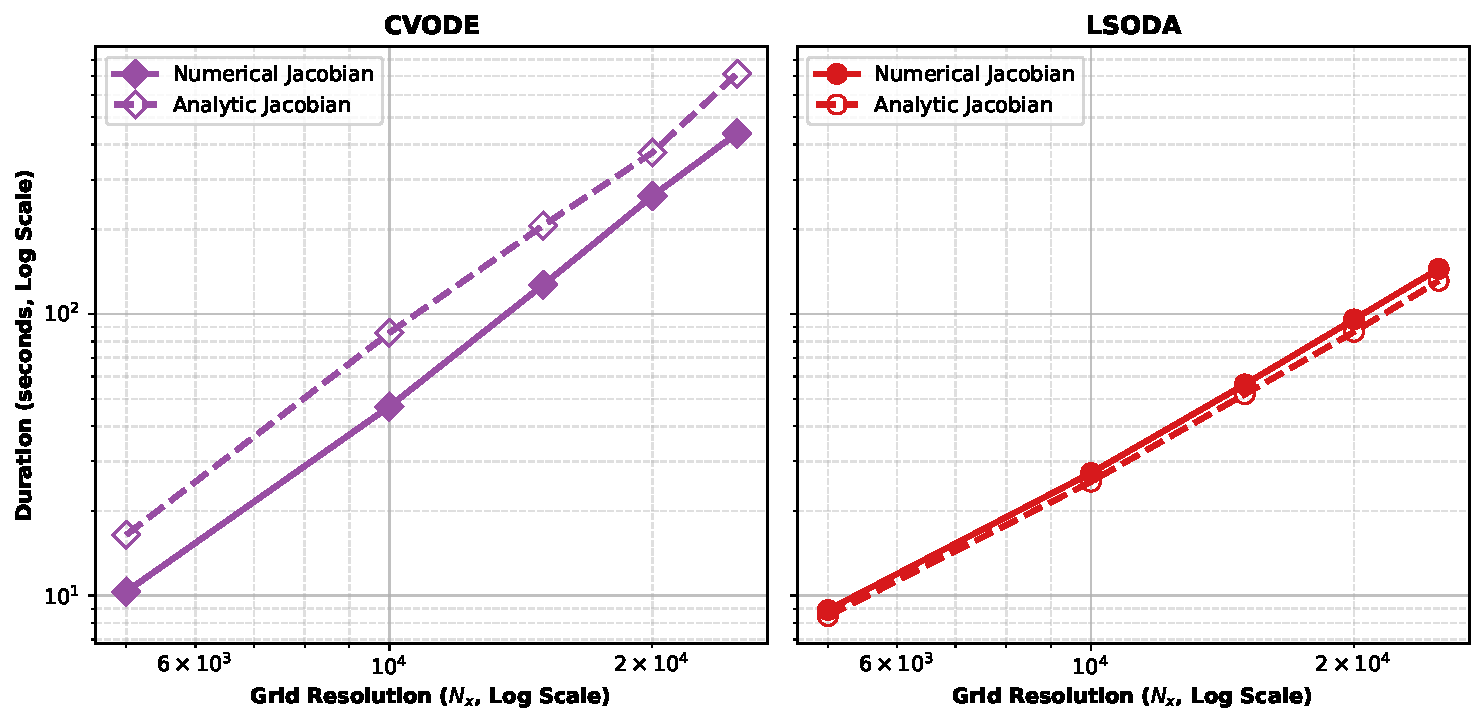
\includegraphics[width=\textwidth]{images/fdm_analytic_comparison_lsoda_cvode.pdf}
  \caption{Analytical vs.\ numerical Jacobian for LSODA and CVODE across grid resolutions (\(p = 4.0\), \(\varepsilon = 10^{-6}\), tolerance \(10^{-6}\)).}
  \label{fig:analytic-lsoda-cvode}
\end{figure}
